\documentclass[12pt,a4paper]{article}
\usepackage[T1]{fontenc}
\usepackage[utf8]{inputenc}
\usepackage{lmodern}
\usepackage{amsmath,amssymb,amsthm,mathtools}
\usepackage{geometry}
\geometry{margin=1in}
\usepackage{microtype}
\usepackage{hyperref}
\usepackage{xcolor}
\usepackage{enumitem}
\usepackage{fancyhdr}
\usepackage{bookmark}

\usepackage{centernot}

\DeclareMathOperator{\rank}{rank}

\DeclareMathOperator{\Deck}{Deck}

\usepackage{tikz-cd}

\usepackage{tocloft}
\setlength{\cftsubsecnumwidth}{3.2em}

\newtheorem{prop}{Proposition}[section]


\newtheorem{definition}{Definition}[section]

\newtheorem{example}[definition]{Example}

\hypersetup{
	colorlinks=true,
	linkcolor=blue!50!black,
	urlcolor=blue!50!black,
	citecolor=blue!50!black,
	pdftitle={Theory of Algebraic Topology 7},
	pdfauthor={},
	pdfsubject={Solved problems and theory notes in commutative algebra},
	pdfcreator={OpenAI}
}

\setlist[itemize]{topsep=4pt,itemsep=2pt,parsep=0pt,partopsep=0pt}
\setlength{\parskip}{0.55em}
\setlength{\parindent}{0pt}

\setcounter{secnumdepth}{2}


\setcounter{tocdepth}{2}

\pagestyle{fancy}


\fancyhf{}
\lhead{Theory of Algebraic Topology 7}
\rhead{\thepage}
\renewcommand{\headrulewidth}{0.4pt}

\newtheoremstyle{notespace}{6pt}{6pt}{\normalfont}{} {\bfseries}{.}{0.5em}{}
\theoremstyle{notespace}

\newtheorem{remark}{Remark}[section]

\DeclareMathOperator{\Spec}{Spec}
\DeclareMathOperator{\Ass}{Ass}
\DeclareMathOperator{\Ann}{Ann}
\DeclareMathOperator{\Supp}{Supp}
\DeclareMathOperator{\Hom}{Hom}
\DeclareMathOperator{\Min}{Min}
\DeclareMathOperator{\Ker}{Ker}
\DeclareMathOperator{\Frac}{Frac}

\DeclareMathOperator{\depth}{depth}
\DeclareMathOperator{\Tor}{Tor}
\DeclareMathOperator{\Ext}{Ext}

\DeclareMathOperator{\coker}{coker}
\DeclareMathOperator{\im}{im}

\newcommand{\longdash}{\mathrel{\text{---}}}

\title{\vspace{-1.5em}\bfseries Theory of Algebraic Topology 7}
\author{}
\date{\today}

\begin{document}
	\maketitle
	\thispagestyle{plain}
		\begin{center}
		\begin{minipage}{0.92\textwidth}
			Lecture notes with worked examples in algebraic topology
		\end{minipage}
	\end{center}
		\pdfbookmark[1]{Contents}{contents}\tableofcontents
	\clearpage

\section{Homology and the idea of holes}

A good first slogan is:

\[
H_k(X) \text{ measures } k\text{-dimensional holes in } X.
\]

This is better than saying that \(H_k\) counts \((k-1)\)-dimensional holes.

More concretely:

\begin{itemize}
	\item \(H_0(X)\): connected components,
	\item \(H_1(X)\): loops, tunnels, or \(1\)-dimensional holes,
	\item \(H_2(X)\): shells or cavities bounded by surfaces,
	\item \(H_3(X)\): higher-dimensional enclosed voids.
\end{itemize}

Strictly speaking, homology groups do not only give a number of holes; they are groups, and may also contain torsion. However, the rank of \(H_k(X)\) gives the number of independent \(k\)-dimensional holes.

\subsection{Basic examples}

\begin{itemize}
	\item For the circle \(S^1\),
	\[
	H_1(S^1)=\mathbb Z.
	\]
	This means there is one basic \(1\)-dimensional hole.
	
	\item For the sphere \(S^2\),
	\[
	H_1(S^2)=0,
	\qquad
	H_2(S^2)=\mathbb Z.
	\]
	So the sphere has no essential loop-holes, but it has one essential \(2\)-dimensional shell.
	
	\item For the torus \(T^2\),
	\[
	H_1(T^2)=\mathbb Z^2,
	\qquad
	H_2(T^2)=\mathbb Z.
	\]
	Thus the torus has two independent \(1\)-dimensional holes and one \(2\)-dimensional fundamental surface class.
	
	\item For the \(3\)-sphere \(S^3\),
	\[
	H_3(S^3)=\mathbb Z.
	\]
	This is the higher-dimensional analogue of the fact that \(H_1(S^1)=\mathbb Z\) and \(H_2(S^2)=\mathbb Z\).
\end{itemize}

\subsection{Why does the circle have \(H_1(S^1)=\mathbb Z\)?}

This is a very important question. If the circle has ``one hole,'' why is the answer \(\mathbb Z\) and not just \(1\)?

The reason is that homology does not merely record the existence of a hole. It records all possible \(1\)-cycles up to boundaries, and these cycles can go around the circle any integer number of times.

\subsubsection{Geometric explanation}

Let \(\gamma\) be the class of a loop that goes once around the circle in the positive direction. Then:

\begin{itemize}
	\item going once around gives the class \([\gamma]\),
	\item going twice around gives \(2[\gamma]\),
	\item going \(n\) times around gives \(n[\gamma]\),
	\item going in the opposite direction gives \(-[\gamma]\).
\end{itemize}

So the possible homology classes are

\[
\ldots,-2[\gamma],-1[\gamma],0,[\gamma],2[\gamma],3[\gamma],\ldots
\]

These are naturally indexed by the integers. Therefore,

\[
H_1(S^1)\cong \mathbb Z.
\]

So \(\mathbb Z\) appears because:
\begin{enumerate}
	\item there is one basic loop-generator,
	\item it may be traversed any integer number of times,
	\item orientation matters, so negative integers also appear.
\end{enumerate}

\subsubsection{Chain-complex computation}

We can also see this algebraically by giving \(S^1\) a cell structure with one vertex \(v\) and one oriented edge \(e\) whose endpoints are both attached to \(v\).

Then the chain groups are

\[
C_1 \cong \mathbb Z\langle e\rangle \cong \mathbb Z,
\qquad
C_0 \cong \mathbb Z\langle v\rangle \cong \mathbb Z,
\qquad
C_2=0.
\]

The boundary map is

\[
\partial_1(e)=v-v=0,
\]

because the beginning and endpoint of the edge are the same vertex.

Hence

\[
\ker(\partial_1)=C_1\cong \mathbb Z.
\]

Also, since \(C_2=0\), we have

\[
\operatorname{im}(\partial_2)=0.
\]

Therefore,

\[
H_1(S^1)
=
\frac{\ker(\partial_1)}{\operatorname{im}(\partial_2)}
=
\frac{\mathbb Z}{0}
=
\mathbb Z.
\]

\subsubsection{Interpretation}

Thus the circle has one fundamental \(1\)-dimensional hole, but the homology group is \(\mathbb Z\) because the basic loop can be taken with arbitrary integer multiplicity.

So:

\[
\text{``one hole''} \quad \Longrightarrow \quad \text{one generator of } H_1,
\]

and one generator means

\[
H_1(S^1)\cong \mathbb Z,
\]

not just the number \(1\).

\subsection{A useful summary}

\[
\begin{array}{c|c|c|c}
	X & H_1(X) & H_2(X) & H_3(X) \\
	\hline
	S^1 & \mathbb Z & 0 & 0 \\
	S^2 & 0 & \mathbb Z & 0 \\
	T^2 & \mathbb Z^2 & \mathbb Z & 0 \\
	S^3 & 0 & 0 & \mathbb Z
\end{array}
\]

The main idea is:

\begin{quote}
	\(H_k(X)\) detects \(k\)-dimensional cycles modulo boundaries, and its rank counts the number of independent \(k\)-dimensional holes.
\end{quote}

\subsection{Concrete geometric explanations of
	\texorpdfstring{$H_1(T^2)=\mathbb Z^2$, $H_2(S^2)=\mathbb Z$, and $H_1(\mathbb{RP}^2)=\mathbb Z/2$}{H1(T2)=Z2, H2(S2)=Z, H1(RP2)=Z/2}} 

We now explain three standard examples very concretely.

\subsubsection{Why \texorpdfstring{$H_1(T^2)=\mathbb Z^2$}{H1(T2)=Z2}}

Think of the torus \(T^2\) as the surface of a donut.

There are two basic kinds of essential loops on a torus:

\begin{itemize}
	\item one loop goes around the central hole of the donut,
	\item one loop goes around the tube itself.
\end{itemize}

Call their homology classes \(a\) and \(b\).

These two loops are independent:

\begin{itemize}
	\item \(a\) cannot be deformed into \(b\),
	\item neither \(a\) nor \(b\) is the boundary of a \(2\)-dimensional region inside the torus,
	\item any \(1\)-cycle on the torus is homologous to some combination
	\[
	m a + n b, \qquad m,n\in\mathbb Z.
	\]
\end{itemize}

So every homology class in \(H_1(T^2)\) is determined by two integers: how many times we go around in the \(a\)-direction and how many times we go around in the \(b\)-direction.

Therefore,
\[
H_1(T^2)\cong \mathbb Z\oplus \mathbb Z=\mathbb Z^2.
\]

\paragraph{Square model of the torus.}
Another very useful picture is the quotient square model of the torus:
opposite horizontal edges are identified, and opposite vertical edges are identified.

Then the two edge directions give two basic loops:
\[
a=\text{horizontal loop}, \qquad b=\text{vertical loop}.
\]

The interior of the square becomes the \(2\)-cell of the torus, but its boundary word is
\[
aba^{-1}b^{-1}.
\]

In homology, order does not matter and inverses become negatives, so
\[
a+b-a-b=0.
\]

Thus the \(2\)-cell contributes no nontrivial relation in \(H_1\), and the two generators \(a,b\) survive independently. Hence
\[
H_1(T^2)=\mathbb Z^2.
\]

\paragraph{Interpretation.}
So the torus has two independent \(1\)-dimensional holes, and that is why the first homology group is \(\mathbb Z^2\).

\subsubsection{Why \texorpdfstring{$H_2(S^2)=\mathbb Z$}{H2(S2)=Z}}

Now consider the sphere \(S^2\).

A sphere has no essential \(1\)-dimensional loop-holes, because every loop on a sphere can be shrunk to a point. So
\[
H_1(S^2)=0.
\]

However, the whole sphere itself is a closed \(2\)-dimensional surface. It is a \(2\)-cycle: it has no boundary.

This \(2\)-cycle is not the boundary of any \(3\)-chain inside \(S^2\), because the sphere itself is the whole space; there is no \(3\)-dimensional cell in the sphere whose boundary would be the sphere.

Thus the whole oriented sphere gives a nonzero class in \(H_2(S^2)\).

Moreover, every \(2\)-cycle on \(S^2\) is an integer multiple of the fundamental class of the sphere. So all classes look like
\[
n[S^2], \qquad n\in\mathbb Z.
\]

Therefore,
\[
H_2(S^2)\cong \mathbb Z.
\]

\paragraph{CW-complex view.}
We may give \(S^2\) a CW structure with:

\begin{itemize}
	\item one \(0\)-cell \(e^0\),
	\item one \(2\)-cell \(e^2\),
	\item no \(1\)-cells.
\end{itemize}

Then
\[
C_2\cong \mathbb Z,\qquad C_1=0,\qquad C_0\cong \mathbb Z.
\]

Since \(C_1=0\), the boundary map
\[
\partial_2:C_2\to C_1
\]
is zero. Hence
\[
\ker(\partial_2)=C_2\cong \mathbb Z.
\]

Also \(C_3=0\), so
\[
\operatorname{im}(\partial_3)=0.
\]

Therefore,
\[
H_2(S^2)=\frac{\ker(\partial_2)}{\operatorname{im}(\partial_3)}
=\frac{\mathbb Z}{0}
=\mathbb Z.
\]

\paragraph{Interpretation.}
So \(H_2(S^2)=\mathbb Z\) means that the sphere has one basic \(2\)-dimensional shell class, and it can be taken with any integer multiplicity and orientation.

\subsubsection{Why \texorpdfstring{$H_1(\mathbb{RP}^2)=\mathbb Z/2$}{H1(RP2)=Z/2}}

This is the first standard example where torsion appears.

A very concrete model for \(\mathbb{RP}^2\) is:

\begin{quote}
	a disk whose boundary points are identified in antipodal pairs.
\end{quote}

So if \(x\in \partial D^2=S^1\), then \(x\sim -x\).

Geometrically, this means that the boundary circle does not survive as an ordinary full loop. Instead, opposite boundary points are glued together, and this changes the homology relation.

There is one basic \(1\)-dimensional class \(a\), but the boundary of the \(2\)-cell wraps around this loop twice. Therefore,
\[
2a=0
\]
in homology.

That is exactly why the first homology group is not \(\mathbb Z\), but \(\mathbb Z/2\).

\paragraph{CW-complex computation.}
A standard CW structure on \(\mathbb{RP}^2\) has:

\begin{itemize}
	\item one \(0\)-cell \(e^0\),
	\item one \(1\)-cell \(e^1\),
	\item one \(2\)-cell \(e^2\).
\end{itemize}

The \(1\)-cell is attached to the single \(0\)-cell at both ends, so
\[
\partial_1=0.
\]

The \(2\)-cell is attached by a map of degree \(2\) around the \(1\)-skeleton, so
\[
\partial_2:\mathbb Z\to \mathbb Z
\]
is multiplication by \(2\):
\[
\partial_2(1)=2.
\]

Thus
\[
C_2\cong \mathbb Z,\qquad C_1\cong \mathbb Z,\qquad C_0\cong \mathbb Z,
\]
with
\[
\partial_2(n)=2n,\qquad \partial_1=0.
\]

Hence
\[
H_1(\mathbb{RP}^2)
=
\frac{\ker(\partial_1)}{\operatorname{im}(\partial_2)}
=
\frac{\mathbb Z}{2\mathbb Z}
=
\mathbb Z/2.
\]

\paragraph{Geometric interpretation.}
There is one basic loop \(a\), but going around twice becomes a boundary. So:

\begin{itemize}
	\item \(a\neq 0\),
	\item \(2a=0\).
\end{itemize}

Therefore the only homology classes are
\[
0,\ a.
\]

So
\[
H_1(\mathbb{RP}^2)=\mathbb Z/2.
\]

This does \emph{not} mean that \(\mathbb{RP}^2\) has ``half a hole.'' It means the first homology has torsion of order \(2\).

\subsubsection{Summary}

\[
\begin{array}{c|c|c|l}
	X & H_1(X) & H_2(X) & \text{Geometric meaning} \\
	\hline
	T^2 & \mathbb Z^2 & \mathbb Z & \text{two independent loops on the torus} \\
	S^2 & 0 & \mathbb Z & \text{one fundamental spherical shell} \\
	\mathbb{RP}^2 & \mathbb Z/2 & 0 & \text{one loop }a\text{ with }2a=0
\end{array}
\]

So the three key pictures are:

\begin{itemize}
	\item on the torus, there are \emph{two independent} directions for essential loops, hence \(\mathbb Z^2\);
	\item on the sphere, the whole oriented surface is one basic \(2\)-cycle, hence \(\mathbb Z\);
	\item on \(\mathbb{RP}^2\), there is one basic loop, but twice that loop bounds the \(2\)-cell, hence \(\mathbb Z/2\).
\end{itemize}

\subsection{Quotient pictures for the torus and for \texorpdfstring{$\mathbb{RP}^2$}{RP2}}

These pictures are often the fastest way to understand why
\[
H_1(T^2)=\mathbb Z^2
\qquad\text{and}\qquad
H_1(\mathbb{RP}^2)=\mathbb Z/2.
\]

\subsubsection{The torus as a quotient square}

The torus \(T^2\) may be obtained from a square by identifying opposite sides in the same direction.

\begin{figure}[h!]
	\centering
	\begin{tikzpicture}[scale=1.2, >=Latex]
		
		% square
		\draw[thick] (0,0) rectangle (4,4);
		
		% labels
		\node at (2,-0.45) {\(a\)};
		\node at (2,4.45) {\(a\)};
		\node at (-0.45,2) {\(b\)};
		\node at (4.45,2) {\(b\)};
		
		% arrows on horizontal edges
		\draw[->, thick] (0.8,0) -- (3.2,0);
		\draw[->, thick] (0.8,4) -- (3.2,4);
		
		% arrows on vertical edges
		\draw[->, thick] (0,0.8) -- (0,3.2);
		\draw[->, thick] (4,0.8) -- (4,3.2);
		
		% corner labels
		\node[below left] at (0,0) {\small \(v\)};
		\node[below right] at (4,0) {\small \(v\)};
		\node[above left] at (0,4) {\small \(v\)};
		\node[above right] at (4,4) {\small \(v\)};
		
	\end{tikzpicture}
	\caption{A quotient-square model of the torus \(T^2\). Opposite horizontal edges are identified, and opposite vertical edges are identified.}
\end{figure}

Geometrically, after gluing:

\begin{itemize}
	\item the bottom edge and the top edge become one loop, called \(a\),
	\item the left edge and the right edge become another loop, called \(b\),
	\item all four corners become a single vertex \(v\).
\end{itemize}

So the \(1\)-skeleton is a wedge of two circles:
\[
S^1 \vee S^1.
\]

The interior of the square becomes a \(2\)-cell attached along the boundary word
\[
aba^{-1}b^{-1}.
\]

For the fundamental group this relation is important, since it says
\[
ab = ba.
\]

But in homology we abelianize automatically, so the boundary of the \(2\)-cell becomes
\[
a+b-a-b=0.
\]

Thus the \(2\)-cell adds no new nontrivial relation in \(H_1\), and both generators survive independently. Therefore
\[
H_1(T^2)=\mathbb Z\langle a\rangle \oplus \mathbb Z\langle b\rangle \cong \mathbb Z^2.
\]

\paragraph{Geometric meaning.}
The two generators correspond to the two basic essential loops on the torus:

\begin{itemize}
	\item one going around the tube,
	\item one going around the central hole.
\end{itemize}

Any \(1\)-cycle on the torus is homologous to
\[
ma+nb
\qquad (m,n\in\mathbb Z),
\]
so two integers are needed to record its homology class.

\subsubsection{The projective plane as a disk with antipodal boundary points identified}

A very concrete model for \(\mathbb{RP}^2\) is obtained from a disk \(D^2\) by identifying opposite points on the boundary circle.

\[
x \sim -x \qquad \text{for } x\in \partial D^2=S^1.
\]

Equivalently, one may use a square whose boundary is glued according to the word \(aa\).

\begin{figure}[h!]
	\centering
	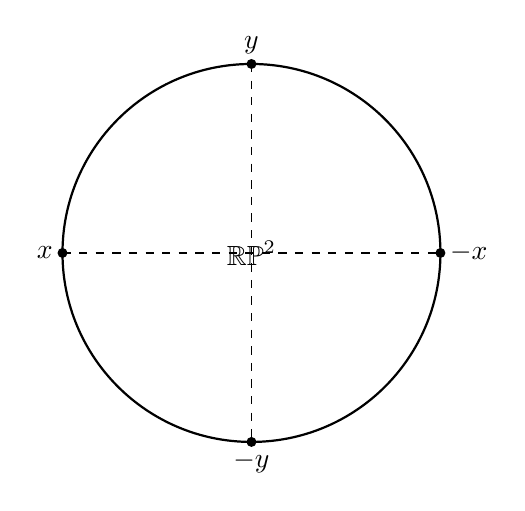
\begin{tikzpicture}[scale=1.2, >=Latex]
		
		% disk
		\draw[thick] (0,0) circle (2);
		
		% center text
		\node at (0,0) {\(\mathbb{RP}^2\)};
		
		% antipodal points
		\fill (-2,0) circle (1.5pt);
		\fill (2,0) circle (1.5pt);
		\fill (0,2) circle (1.5pt);
		\fill (0,-2) circle (1.5pt);
		
		\node[left] at (-2,0) {\(x\)};
		\node[right] at (2,0) {\(-x\)};
		\node[above] at (0,2) {\(y\)};
		\node[below] at (0,-2) {\(-y\)};
		
		% dashed identification hints
		\draw[dashed] (-2,0) -- (2,0);
		\draw[dashed] (0,2) -- (0,-2);
		
	\end{tikzpicture}
	\caption{Disk model of \(\mathbb{RP}^2\): antipodal points of the boundary circle are identified.}
\end{figure}

Another common picture is the quotient square with edge pattern \(aa\):

\begin{figure}[h!]
	\centering
	\begin{tikzpicture}[scale=1.2, >=Latex]
		
		% square
		\draw[thick] (0,0) rectangle (4,4);
		
		% arrows both directions matching for aa picture
		\draw[->, thick] (0.8,0) -- (3.2,0);
		\draw[->, thick] (0.8,4) -- (3.2,4);
		
		% side labels
		\node at (2,-0.45) {\(a\)};
		\node at (2,4.45) {\(a\)};
		
		% corner labels
		\node[below left] at (0,0) {\small \(v_1\)};
		\node[below right] at (4,0) {\small \(v_2\)};
		\node[above left] at (0,4) {\small \(v_2\)};
		\node[above right] at (4,4) {\small \(v_1\)};
		
	\end{tikzpicture}
	\caption{Square model for \(\mathbb{RP}^2\): the two horizontal edges are glued in the same direction, giving boundary word \(aa\).}
\end{figure}

\paragraph{Why does this give \(\mathbb Z/2\)?}

There is one basic \(1\)-dimensional loop \(a\). The key point is that the boundary of the \(2\)-cell goes around that loop twice. Thus
\[
\partial_2(e^2)=2a.
\]

So in the chain complex we have
\[
C_2 \cong \mathbb Z,\qquad C_1 \cong \mathbb Z,\qquad C_0 \cong \mathbb Z,
\]
with
\[
\partial_2(n)=2n,\qquad \partial_1=0.
\]

Therefore
\[
H_1(\mathbb{RP}^2)
=
\frac{\ker(\partial_1)}{\operatorname{im}(\partial_2)}
=
\frac{\mathbb Z}{2\mathbb Z}
=
\mathbb Z/2.
\]

\paragraph{Geometric meaning.}
There is one basic loop \(a\), but twice that loop becomes a boundary:
\[
2a=0.
\]

So there are only two homology classes:
\[
0 \quad\text{and}\quad a.
\]

That is exactly what \(\mathbb Z/2\) means.

\subsubsection{Comparison of the two pictures}

The torus and the projective plane both come from gluing the boundary of a polygon, but the gluing pattern is different.

\begin{itemize}
	\item For the torus, the square has edge word
	\[
	aba^{-1}b^{-1},
	\]
	so two independent \(1\)-cycles survive:
	\[
	H_1(T^2)=\mathbb Z^2.
	\]
	
	\item For \(\mathbb{RP}^2\), the square has edge word
	\[
	aa,
	\]
	so one generator \(a\) survives, but with relation
	\[
	2a=0,
	\]
	hence
	\[
	H_1(\mathbb{RP}^2)=\mathbb Z/2.
	\]
\end{itemize}

\subsubsection{Very short intuition}

\begin{itemize}
	\item Torus: two independent directions of going around \(\Rightarrow \mathbb Z^2\).
	\item Projective plane: one basic loop, but going around twice bounds the \(2\)-cell \(\Rightarrow \mathbb Z/2\).
\end{itemize}

\subsection{Quotient pictures for the torus and for \texorpdfstring{$\mathbb{RP}^2$}{RP2}}

These pictures are often the fastest way to understand why
\[
H_1(T^2)=\mathbb Z^2
\qquad\text{and}\qquad
H_1(\mathbb{RP}^2)=\mathbb Z/2.
\]

\subsubsection{The torus as a quotient square}

The torus \(T^2\) may be obtained from a square by identifying opposite sides in the same direction.

\begin{figure}[h!]
	\centering
	\begin{tikzpicture}[scale=1.2, >=Latex]
		
		% square
		\draw[thick] (0,0) rectangle (4,4);
		
		% labels
		\node at (2,-0.45) {\(a\)};
		\node at (2,4.45) {\(a\)};
		\node at (-0.45,2) {\(b\)};
		\node at (4.45,2) {\(b\)};
		
		% arrows on horizontal edges
		\draw[->, thick] (0.8,0) -- (3.2,0);
		\draw[->, thick] (0.8,4) -- (3.2,4);
		
		% arrows on vertical edges
		\draw[->, thick] (0,0.8) -- (0,3.2);
		\draw[->, thick] (4,0.8) -- (4,3.2);
		
		% corner labels
		\node[below left] at (0,0) {\small \(v\)};
		\node[below right] at (4,0) {\small \(v\)};
		\node[above left] at (0,4) {\small \(v\)};
		\node[above right] at (4,4) {\small \(v\)};
		
	\end{tikzpicture}
	\caption{A quotient-square model of the torus \(T^2\). Opposite horizontal edges are identified, and opposite vertical edges are identified.}
\end{figure}

Geometrically, after gluing:

\begin{itemize}
	\item the bottom edge and the top edge become one loop, called \(a\),
	\item the left edge and the right edge become another loop, called \(b\),
	\item all four corners become a single vertex \(v\).
\end{itemize}

So the \(1\)-skeleton is a wedge of two circles:
\[
S^1 \vee S^1.
\]

The interior of the square becomes a \(2\)-cell attached along the boundary word
\[
aba^{-1}b^{-1}.
\]

For the fundamental group this relation is important, since it says
\[
ab = ba.
\]

But in homology we abelianize automatically, so the boundary of the \(2\)-cell becomes
\[
a+b-a-b=0.
\]

Thus the \(2\)-cell adds no new nontrivial relation in \(H_1\), and both generators survive independently. Therefore
\[
H_1(T^2)=\mathbb Z\langle a\rangle \oplus \mathbb Z\langle b\rangle \cong \mathbb Z^2.
\]

\paragraph{Geometric meaning.}
The two generators correspond to the two basic essential loops on the torus:

\begin{itemize}
	\item one going around the tube,
	\item one going around the central hole.
\end{itemize}

Any \(1\)-cycle on the torus is homologous to
\[
ma+nb
\qquad (m,n\in\mathbb Z),
\]
so two integers are needed to record its homology class.

\subsubsection{The projective plane as a disk with antipodal boundary points identified}

A very concrete model for \(\mathbb{RP}^2\) is obtained from a disk \(D^2\) by identifying opposite points on the boundary circle.

\[
x \sim -x \qquad \text{for } x\in \partial D^2=S^1.
\]

Equivalently, one may use a square whose boundary is glued according to the word \(aa\).

\begin{figure}[h!]
	\centering
	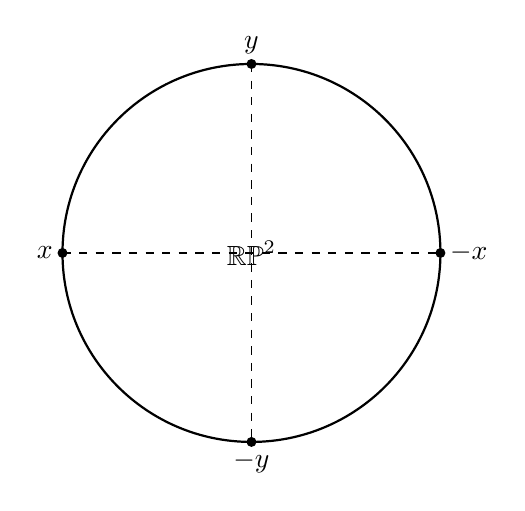
\begin{tikzpicture}[scale=1.2, >=Latex]
		
		% disk
		\draw[thick] (0,0) circle (2);
		
		% center text
		\node at (0,0) {\(\mathbb{RP}^2\)};
		
		% antipodal points
		\fill (-2,0) circle (1.5pt);
		\fill (2,0) circle (1.5pt);
		\fill (0,2) circle (1.5pt);
		\fill (0,-2) circle (1.5pt);
		
		\node[left] at (-2,0) {\(x\)};
		\node[right] at (2,0) {\(-x\)};
		\node[above] at (0,2) {\(y\)};
		\node[below] at (0,-2) {\(-y\)};
		
		% dashed identification hints
		\draw[dashed] (-2,0) -- (2,0);
		\draw[dashed] (0,2) -- (0,-2);
		
	\end{tikzpicture}
	\caption{Disk model of \(\mathbb{RP}^2\): antipodal points of the boundary circle are identified.}
\end{figure}

Another common picture is the quotient square with edge pattern \(aa\):

\begin{figure}[h!]
	\centering
	\begin{tikzpicture}[scale=1.2, >=Latex]
		
		% square
		\draw[thick] (0,0) rectangle (4,4);
		
		% arrows both directions matching for aa picture
		\draw[->, thick] (0.8,0) -- (3.2,0);
		\draw[->, thick] (0.8,4) -- (3.2,4);
		
		% side labels
		\node at (2,-0.45) {\(a\)};
		\node at (2,4.45) {\(a\)};
		
		% corner labels
		\node[below left] at (0,0) {\small \(v_1\)};
		\node[below right] at (4,0) {\small \(v_2\)};
		\node[above left] at (0,4) {\small \(v_2\)};
		\node[above right] at (4,4) {\small \(v_1\)};
		
	\end{tikzpicture}
	\caption{Square model for \(\mathbb{RP}^2\): the two horizontal edges are glued in the same direction, giving boundary word \(aa\).}
\end{figure}

\paragraph{Why does this give \(\mathbb Z/2\)?}

There is one basic \(1\)-dimensional loop \(a\). The key point is that the boundary of the \(2\)-cell goes around that loop twice. Thus
\[
\partial_2(e^2)=2a.
\]

So in the chain complex we have
\[
C_2 \cong \mathbb Z,\qquad C_1 \cong \mathbb Z,\qquad C_0 \cong \mathbb Z,
\]
with
\[
\partial_2(n)=2n,\qquad \partial_1=0.
\]

Therefore
\[
H_1(\mathbb{RP}^2)
=
\frac{\ker(\partial_1)}{\operatorname{im}(\partial_2)}
=
\frac{\mathbb Z}{2\mathbb Z}
=
\mathbb Z/2.
\]

\paragraph{Geometric meaning.}
There is one basic loop \(a\), but twice that loop becomes a boundary:
\[
2a=0.
\]

So there are only two homology classes:
\[
0 \quad\text{and}\quad a.
\]

That is exactly what \(\mathbb Z/2\) means.

\subsubsection{Comparison of the two pictures}

The torus and the projective plane both come from gluing the boundary of a polygon, but the gluing pattern is different.

\begin{itemize}
	\item For the torus, the square has edge word
	\[
	aba^{-1}b^{-1},
	\]
	so two independent \(1\)-cycles survive:
	\[
	H_1(T^2)=\mathbb Z^2.
	\]
	
	\item For \(\mathbb{RP}^2\), the square has edge word
	\[
	aa,
	\]
	so one generator \(a\) survives, but with relation
	\[
	2a=0,
	\]
	hence
	\[
	H_1(\mathbb{RP}^2)=\mathbb Z/2.
	\]
\end{itemize}

\subsubsection{Very short intuition}

\begin{itemize}
	\item Torus: two independent directions of going around \(\Rightarrow \mathbb Z^2\).
	\item Projective plane: one basic loop, but going around twice bounds the \(2\)-cell \(\Rightarrow \mathbb Z/2\).
\end{itemize}

\section{Singular, simplicial, cellular, and de Rham theories}

There are several standard homology and cohomology theories in topology and geometry. They are closely related, but they are built from different kinds of data and are most useful in different settings.

A very important point is that one should distinguish between \emph{homology} and \emph{cohomology}. In particular, de Rham theory is usually a theory of \emph{cohomology}, not homology.

\subsection{ General picture}

The main theories relevant here are:

\begin{itemize}
	\item \textbf{singular homology},
	\item \textbf{simplicial homology},
	\item \textbf{cellular homology},
	\item \textbf{de Rham cohomology}.
\end{itemize}

The first three are homology theories:
\[
H_k(X).
\]

The last one is a cohomology theory:
\[
H^k_{\mathrm{dR}}(M).
\]

Although they are defined differently, they often recover the same topological information when the space is sufficiently nice.

\subsection{ Singular homology}

\subsubsection{Definition}

Singular homology is the most general standard homology theory in algebraic topology.

For a topological space \(X\), a \emph{singular \(k\)-simplex} is a continuous map
\[
\sigma:\Delta^k\to X,
\]
where \(\Delta^k\) is the standard \(k\)-simplex.

The group \(C_k^{\mathrm{sing}}(X)\) of singular \(k\)-chains is the free abelian group generated by all singular \(k\)-simplices:
\[
C_k^{\mathrm{sing}}(X)=\bigoplus_{\sigma:\Delta^k\to X}\mathbb Z\langle \sigma\rangle.
\]

The boundary map is defined by restricting to the faces:
\[
\partial_k(\sigma)=\sum_{i=0}^k(-1)^i\,\sigma|_{[v_0,\dots,\widehat{v_i},\dots,v_k]}.
\]

Thus one gets a chain complex
\[
\cdots \to C_2^{\mathrm{sing}}(X)\xrightarrow{\partial_2}
C_1^{\mathrm{sing}}(X)\xrightarrow{\partial_1}
C_0^{\mathrm{sing}}(X)\to 0.
\]

The singular homology groups are then defined by
\[
H_k^{\mathrm{sing}}(X)=\frac{\ker(\partial_k)}{\operatorname{im}(\partial_{k+1})}.
\]

\subsubsection{Why it is important}

Singular homology is defined for \emph{every} topological space. This is its main advantage. It is the standard general theory, and when one simply writes \(H_k(X)\), one often means singular homology.

\subsubsection{Disadvantage}

It is usually too large for direct computations, because there are enormously many continuous maps \(\Delta^k\to X\).

\subsection{3. Simplicial homology}

\subsubsection{Definition}

Simplicial homology is defined when the space is given as a \emph{simplicial complex} \(K\), or more generally when the space admits a triangulation.

In this case, the \(k\)-chains are formal integer combinations of the oriented \(k\)-simplices already present in the complex:
\[
C_k^{\mathrm{simp}}(K)=\bigoplus_{\sigma\in K^{(k)}} \mathbb Z\langle \sigma\rangle.
\]

The boundary map is the usual alternating sum of faces. For an oriented simplex \([v_0v_1\dots v_k]\),
\[
\partial_k([v_0v_1\dots v_k])
=
\sum_{i=0}^k (-1)^i [v_0\dots \widehat{v_i}\dots v_k].
\]

The simplicial homology groups are
\[
H_k^{\mathrm{simp}}(K)=\frac{\ker(\partial_k)}{\operatorname{im}(\partial_{k+1})}.
\]

\subsubsection{Why it is useful}

Simplicial homology is very concrete and combinatorial. If a space is triangulated, then homology may often be computed directly from the finite list of simplices.

\subsubsection{Relation to singular homology}

If \(X\) is the polyhedron of a simplicial complex \(K\), then
\[
H_k^{\mathrm{simp}}(K)\cong H_k^{\mathrm{sing}}(X).
\]

So simplicial homology is not a different invariant in that setting; it is a more computable model for the same homology.

\subsection{ Cellular homology}

\subsubsection{Definition}

Cellular homology is defined for a \emph{CW-complex} \(X\).

If \(X\) has \(k\)-cells \(e^k_\alpha\), then the cellular chain group is
\[
C_k^{\mathrm{cell}}(X)\cong \bigoplus_\alpha \mathbb Z\langle e^k_\alpha\rangle.
\]

The boundary maps are determined by the attaching maps of the cells. In practice, these boundary maps are often much smaller and easier to compute than the singular chain maps.

The cellular homology groups are
\[
H_k^{\mathrm{cell}}(X)=\frac{\ker(\partial_k)}{\operatorname{im}(\partial_{k+1})}.
\]

\subsubsection{Why it is useful}

For spaces built naturally from cells, this is often the most efficient way to compute homology.

Typical examples are:
\[
S^n,\qquad T^2,\qquad \mathbb{RP}^n,\qquad \mathbb{CP}^n.
\]

For instance:

\begin{itemize}
	\item \(S^1\) has one \(0\)-cell and one \(1\)-cell,
	\item \(S^2\) has one \(0\)-cell and one \(2\)-cell,
	\item \(\mathbb{RP}^2\) has one \(0\)-cell, one \(1\)-cell, and one \(2\)-cell.
\end{itemize}

\subsubsection{Relation to singular homology}

For a CW-complex \(X\),
\[
H_k^{\mathrm{cell}}(X)\cong H_k^{\mathrm{sing}}(X).
\]

So again, cellular homology computes the same homology groups, but from a smaller chain complex.

\subsection{ de Rham cohomology}

\subsubsection{Definition}

de Rham theory is a theory of \emph{cohomology} for smooth manifolds.

If \(M\) is a smooth manifold, let \(\Omega^k(M)\) be the space of smooth differential \(k\)-forms on \(M\). The exterior derivative
\[
d:\Omega^k(M)\to \Omega^{k+1}(M)
\]
satisfies
\[
d\circ d=0.
\]

Thus the differential forms form a cochain complex
\[
0\to \Omega^0(M)\xrightarrow{d}\Omega^1(M)\xrightarrow{d}\Omega^2(M)\xrightarrow{d}\cdots.
\]

The \(k\)-th de Rham cohomology group is
\[
H^k_{\mathrm{dR}}(M)
=
\frac{\ker\bigl(d:\Omega^k(M)\to \Omega^{k+1}(M)\bigr)}
{\operatorname{im}\bigl(d:\Omega^{k-1}(M)\to \Omega^k(M)\bigr)}.
\]

So:

\begin{itemize}
	\item the numerator consists of \emph{closed forms},
	\item the denominator consists of \emph{exact forms}.
\end{itemize}

\subsubsection{Why it is different}

This is cohomology, not homology. Also, it uses differential forms, so it requires smooth structure.

\subsubsection{Relation to singular cohomology}

The de Rham theorem says that for a smooth manifold \(M\),
\[
H^k_{\mathrm{dR}}(M)\cong H^k_{\mathrm{sing}}(M;\mathbb R),
\]
that is, de Rham cohomology is naturally isomorphic to singular cohomology with real coefficients.

So de Rham cohomology gives the same cohomological information as singular cohomology over \(\mathbb R\), but in a differential-geometric form.

\subsection{ Why ``complex'' is not one more homology theory}

Sometimes one hears words such as:

\begin{itemize}
	\item simplicial complex,
	\item chain complex,
	\item CW-complex.
\end{itemize}

But the word \emph{complex} by itself does not name one extra homology theory.

Instead:

\begin{itemize}
	\item a \textbf{simplicial complex} is a combinatorial object built from simplices,
	\item a \textbf{CW-complex} is a space built by attaching cells,
	\item a \textbf{chain complex} is an algebraic sequence
	\[
	\cdots \to C_{k+1}\xrightarrow{\partial_{k+1}} C_k\xrightarrow{\partial_k} C_{k-1}\to\cdots
	\]
	with \(\partial_k\circ\partial_{k+1}=0\).
\end{itemize}

Homology is then constructed from a chain complex by
\[
H_k=\frac{\ker(\partial_k)}{\operatorname{im}(\partial_{k+1})}.
\]

So ``complex'' refers to the structure from which homology is computed, not usually to a separate theory.

\subsection{ Comparison of the theories}

\[
\begin{array}{c|c|c|c}
	\text{Theory} & \text{Built from} & \text{Defined for} & \text{Output} \\
	\hline
	\text{Singular homology} & \text{all continuous simplices} & \text{all topological spaces} & H_k(X) \\[4pt]
	\text{Simplicial homology} & \text{simplices in a triangulation} & \text{simplicial complexes} & H_k(X) \\[4pt]
	\text{Cellular homology} & \text{cells and attaching maps} & \text{CW-complexes} & H_k(X) \\[4pt]
	\text{de Rham cohomology} & \text{differential forms} & \text{smooth manifolds} & H^k_{\mathrm{dR}}(M)
\end{array}
\]

\subsection{ Agreement of the theories}

When the space is sufficiently nice, these theories agree in the expected way.

\begin{itemize}
	\item If \(X\) is triangulated by a simplicial complex \(K\), then
	\[
	H_k^{\mathrm{simp}}(K)\cong H_k^{\mathrm{sing}}(X).
	\]
	
	\item If \(X\) is a CW-complex, then
	\[
	H_k^{\mathrm{cell}}(X)\cong H_k^{\mathrm{sing}}(X).
	\]
	
	\item If \(M\) is a smooth manifold, then
	\[
	H^k_{\mathrm{dR}}(M)\cong H^k_{\mathrm{sing}}(M;\mathbb R).
	\]
\end{itemize}

So, in good situations, these are different computational models for the same topological information.

\subsection{ Example: the circle \texorpdfstring{$S^1$}{S1}}

The circle is a good example because all the theories can be seen explicitly.

\subsubsection{Singular homology}

Using singular chains, one gets
\[
H_1^{\mathrm{sing}}(S^1)\cong \mathbb Z.
\]

\subsubsection{Simplicial homology}

Triangulate \(S^1\) by a polygon. Then simplicial homology gives
\[
H_1^{\mathrm{simp}}(S^1)\cong \mathbb Z.
\]

\subsubsection{Cellular homology}

Give \(S^1\) a CW structure with one \(0\)-cell and one \(1\)-cell. Then
\[
H_1^{\mathrm{cell}}(S^1)\cong \mathbb Z.
\]

\subsubsection{de Rham cohomology}

For the smooth manifold \(S^1\),
\[
H^1_{\mathrm{dR}}(S^1)\cong \mathbb R.
\]

This does not contradict the homology result \(\mathbb Z\), because:

\begin{itemize}
	\item homology and cohomology are different objects,
	\item de Rham cohomology corresponds to singular cohomology with real coefficients.
\end{itemize}

Indeed,
\[
H^1_{\mathrm{sing}}(S^1;\mathbb R)\cong \mathbb R.
\]

\subsection{ Example: the sphere \texorpdfstring{$S^2$}{S2}}

Similarly, for the sphere:

\begin{itemize}
	\item singular homology gives
	\[
	H_2^{\mathrm{sing}}(S^2)\cong \mathbb Z,
	\]
	\item simplicial homology from any triangulation of the sphere gives
	\[
	H_2^{\mathrm{simp}}(S^2)\cong \mathbb Z,
	\]
	\item cellular homology from one \(0\)-cell and one \(2\)-cell gives
	\[
	H_2^{\mathrm{cell}}(S^2)\cong \mathbb Z,
	\]
	\item de Rham cohomology gives
	\[
	H^2_{\mathrm{dR}}(S^2)\cong \mathbb R.
	\]
\end{itemize}

Again, the last one is real cohomology, not integral homology.

\subsection{ Homology versus cohomology}

It is important not to confuse these.

Homology is built from chains
\[
\cdots \xrightarrow{\partial_{k+1}} C_k \xrightarrow{\partial_k} C_{k-1}\xrightarrow{\partial_{k-1}}\cdots
\]
and gives
\[
H_k=\frac{\ker(\partial_k)}{\operatorname{im}(\partial_{k+1})}.
\]

Cohomology is built from cochains
\[
\cdots \xleftarrow{d^{k+1}} C^k \xleftarrow{d^k} C^{k-1}\xleftarrow{d^{k-1}}\cdots
\]
and gives
\[
H^k=\frac{\ker(d^k)}{\operatorname{im}(d^{k-1})}.
\]

So the notation is different:

\[
H_k \qquad \text{for homology},
\qquad
H^k \qquad \text{for cohomology}.
\]

This is why one writes
\[
H_k^{\mathrm{sing}}(X),\quad H_k^{\mathrm{simp}}(X),\quad H_k^{\mathrm{cell}}(X),
\]
but
\[
H^k_{\mathrm{dR}}(M).
\]

\subsection{ Final summary}

The clean picture is the following.

\begin{itemize}
	\item \textbf{Singular homology} is the most general standard homology theory and works for all topological spaces.
	
	\item \textbf{Simplicial homology} is a combinatorial version for triangulated spaces.
	
	\item \textbf{Cellular homology} is an efficient version for CW-complexes.
	
	\item \textbf{de Rham cohomology} is a differential-form version of real cohomology on smooth manifolds.
	
	\item In the appropriate settings, these theories agree up to natural isomorphism:
	\[
	H_k^{\mathrm{simp}}\cong H_k^{\mathrm{sing}},
	\qquad
	H_k^{\mathrm{cell}}\cong H_k^{\mathrm{sing}},
	\qquad
	H^k_{\mathrm{dR}}\cong H^k_{\mathrm{sing}}(-;\mathbb R).
	\]
\end{itemize}

So one should say:

\begin{quote}
	There are several standard homology and cohomology theories, among them singular homology, simplicial homology, cellular homology, and de Rham cohomology.
\end{quote}

This is the correct refined version of the informal statement that there are ``many kinds of homology.''

\section{Cycles and boundaries: informal discussion with many examples}

Explicit constructions of homology groups are algebraic and can look technical at first. The basic pattern is always the same: one starts with a chain complex
\[
\cdots \xrightarrow{d_{n+1}} C_n \xrightarrow{d_n} C_{n-1} \xrightarrow{d_{n-1}} \cdots
\]
in which each \(C_n\) is an abelian group and the boundary maps satisfy
\[
d_{n-1}\circ d_n = 0
\qquad \text{for all } n.
\]

Homology is then defined by
\[
H_n(X)=\frac{Z_n}{B_n}
=
\frac{\ker d_n}{\operatorname{im} d_{n+1}},
\]
where
\[
Z_n:=\ker d_n
\qquad \text{and} \qquad
B_n:=\operatorname{im} d_{n+1}.
\]

The algebraic meaning is simple:

\begin{itemize}
	\item \(Z_n\) consists of \emph{\(n\)-cycles}, that is, \(n\)-chains whose boundary is zero;
	\item \(B_n\) consists of \emph{\(n\)-boundaries}, that is, \(n\)-chains that arise as the boundary of an \((n+1)\)-chain.
\end{itemize}

So homology measures:

\begin{quote}
	cycles modulo boundaries.
\end{quote}

Equivalently, homology keeps track of closed objects that do \emph{not} already bound something one dimension higher.

\subsection{ The algebraic definitions}

Let
\[
d_n:C_n\to C_{n-1}
\]
be the boundary map. Then:

\[
Z_n=\ker d_n=\{c\in C_n \mid d_n(c)=0\}
\]
is the group of \(n\)-cycles, and

\[
B_n=\operatorname{im} d_{n+1}
=
\{d_{n+1}(c)\mid c\in C_{n+1}\}
\]
is the group of \(n\)-boundaries.

Because
\[
d_n\circ d_{n+1}=0,
\]
every boundary is automatically a cycle:
\[
B_n\subseteq Z_n.
\]

That is why the quotient
\[
H_n=\frac{Z_n}{B_n}
\]
makes sense.

\subsection{ Informal geometric meaning}

The formal definitions above have a very natural geometric interpretation.

\begin{itemize}
	\item A \textbf{boundary} is something that is the edge, rim, shell, or outer limit of a higher-dimensional object.
	\item A \textbf{cycle} is something closed: it has no boundary.
\end{itemize}

Examples from ordinary geometry:

\begin{itemize}
	\item the boundary of the closed interval \([0,1]\) is its two endpoints,
	\item the boundary of a disk \(D^2\) is a circle \(S^1\),
	\item the boundary of a solid ball \(D^3\) is a sphere \(S^2\).
\end{itemize}

Thus:

\begin{itemize}
	\item \(S^1\) is a cycle because it is closed,
	\item \(S^1\) is also a boundary if it appears as \(\partial D^2\),
	\item \(S^2\) is a cycle because it is closed,
	\item \(S^2\) is also a boundary if it appears as \(\partial D^3\).
\end{itemize}

Homology asks whether such cycles bound \emph{inside the given space}. That is crucial.

\subsection{ First example: the interval}

Consider the oriented interval \([0,1]\). Its topological boundary is
\[
\partial [0,1]=\{0\}\amalg \{1\}.
\]

With orientation taken into account, the chain-theoretic boundary is
\[
d_1([0,1])=\{1\}-\{0\}.
\]

More generally, for any integer \(k\),
\[
d_1\bigl(k\cdot [0,1]\bigr)=k\cdot \{1\}-k\cdot \{0\}.
\]

This is the simplest model of the boundary operator: the boundary of an oriented edge is its endpoint minus its starting point.

\paragraph{Why is this useful?}
It shows at once that an interval is not a cycle, because
\[
d_1([0,1])\neq 0.
\]

So an interval has boundary; it is not closed.

\subsection{ Closed loops as cycles}

Now consider a loop obtained by going around a circle once. Informally, this loop has no endpoints, so it should be a cycle.

That is exactly what happens algebraically.

If \(S^1\) is given a CW-structure with one \(0\)-cell \(v\) and one \(1\)-cell \(e\), then
\[
d_1(e)=v-v=0.
\]

Hence \(e\in Z_1\), so \(e\) is a \(1\)-cycle.

Geometrically:

\begin{itemize}
	\item an interval is not closed, so it is not a cycle;
	\item a circle is closed, so it is a cycle.
\end{itemize}

This is the first model for the slogan:

\begin{quote}
	cycles are closed chains.
\end{quote}

\subsection{ A boundary can also be a cycle}

A boundary is always a cycle. This is one of the most important facts.

For example, the boundary of a triangle is
\[
d_2([v_0v_1v_2])
=
[v_1v_2]-[v_0v_2]+[v_0v_1].
\]

This is a closed loop made from three oriented edges. So it is a \(1\)-cycle.

Why must it be a cycle? Because
\[
d_1(d_2([v_0v_1v_2]))=0.
\]

This is a concrete instance of the identity
\[
d_1\circ d_2=0.
\]

So:

\begin{itemize}
	\item the boundary of a triangle is a loop;
	\item that loop is a cycle;
	\item but it is also a boundary, namely the boundary of the triangle itself.
\end{itemize}

This is why homology does not count \emph{all} cycles, only cycles \emph{modulo} boundaries.

\subsection{ Example: the disk and its boundary circle}

Take the closed disk \(D^2\).

Its boundary is the circle:
\[
\partial D^2 = S^1.
\]

So the circle is a \(1\)-cycle, but in the disk it is also a \(1\)-boundary.

Therefore, in the disk, that loop is trivial in homology:
\[
[S^1]=0 \in H_1(D^2).
\]

This matches the geometric intuition: the disk has no \(1\)-dimensional hole. Any loop around its edge bounds the disk.

So the same geometric shape \(S^1\) can behave differently depending on the ambient space:

\begin{itemize}
	\item in \(S^1\) itself, the basic loop does not bound, so it gives a nonzero class in \(H_1(S^1)\);
	\item in \(D^2\), the boundary circle \emph{does} bound, so it becomes zero in \(H_1(D^2)\).
\end{itemize}

\subsection{ Example: the sphere as a \(2\)-cycle}

The sphere \(S^2\) is a closed surface, so it is naturally a \(2\)-cycle.

It has no boundary:
\[
d_2(S^2)=0
\]
in the informal sense that the whole sphere is closed.

But whether it is a boundary depends again on the surrounding space.

\begin{itemize}
	\item In the space \(S^2\) itself, it is not the boundary of any \(3\)-chain, so it gives a nonzero class in \(H_2(S^2)\).
	\item In the solid ball \(D^3\), the sphere \(S^2=\partial D^3\), so there it is a boundary and represents zero in \(H_2(D^3)\).
\end{itemize}

This is an excellent example of the principle:

\begin{quote}
	a cycle may or may not be a boundary, depending on the ambient space.
\end{quote}

\subsection{8. Example: triangle boundary versus filled triangle}

Consider a single filled triangle \(\Delta^2\).

\paragraph{The filled triangle.}
The \(2\)-simplex \([v_0v_1v_2]\) is a \(2\)-chain. It is not a cycle, because
\[
d_2([v_0v_1v_2])\neq 0.
\]

So a filled triangle has boundary.

\paragraph{The edge loop.}
Its boundary
\[
[v_1v_2]-[v_0v_2]+[v_0v_1]
\]
is a \(1\)-cycle, because the endpoints cancel.

So here we see two different things clearly:

\begin{itemize}
	\item the triangle itself is not closed, so it is not a cycle;
	\item the edge loop is closed, so it is a cycle;
	\item but that cycle is also a boundary.
\end{itemize}

\subsection{ Example: a square loop in the plane}

Take four edges forming a square in \(\mathbb R^2\). Their oriented sum forms a closed loop. Hence it is a \(1\)-cycle.

Now ask: is it a boundary?

In the plane \(\mathbb R^2\), yes. It bounds the square region. So in \(\mathbb R^2\), that loop is trivial in first homology.

But if one removes the interior region or modifies the ambient space, the answer may change.

For instance, in the punctured plane
\[
\mathbb R^2\setminus \{0\},
\]
a loop going around the missing point is a \(1\)-cycle that does not bound in that space. Thus it gives a nontrivial homology class.

So:

\begin{itemize}
	\item in \(\mathbb R^2\), loops around ordinary regions are boundaries;
	\item in \(\mathbb R^2\setminus \{0\}\), a loop around the missing point need not be a boundary.
\end{itemize}

This is how holes appear in homology.

\subsection{ Example: the circle \texorpdfstring{$S^1$}{S1}}

The space \(S^1\) itself is the basic example of a nontrivial \(1\)-cycle.

A loop going once around the circle has no boundary, so it lies in \(Z_1\).

But there is no \(2\)-dimensional chain in \(S^1\) whose boundary is that loop. Hence it does not lie in \(B_1\).

Therefore, it defines a nonzero class in
\[
H_1(S^1).
\]

In fact,
\[
H_1(S^1)\cong \mathbb Z,
\]
because one may go around the circle any integer number of times, with sign determined by orientation.

\subsection{ Example: the torus}

The torus \(T^2\) contains many closed loops, hence many \(1\)-cycles.

Among them are two basic ones:

\begin{itemize}
	\item a loop going around the tube,
	\item a loop going around the central hole.
\end{itemize}

Both are cycles, since they are closed.

Neither is a boundary inside the torus.

Therefore both define nontrivial classes in \(H_1(T^2)\), and in fact
\[
H_1(T^2)\cong \mathbb Z^2.
\]

But the torus itself, as a closed surface, is also a \(2\)-cycle. Since it does not bound any \(3\)-chain inside \(T^2\), it gives a nontrivial class in
\[
H_2(T^2)\cong \mathbb Z.
\]

So the torus provides examples in two different dimensions:

\begin{itemize}
	\item nontrivial \(1\)-cycles,
	\item a nontrivial \(2\)-cycle.
\end{itemize}

\subsection{ Example: annulus}

The annulus
\[
A=\{x\in \mathbb R^2 : 1\leq \|x\|\leq 2\}
\]
has two boundary circles as a manifold with boundary:

\[
\partial A = S^1_{\text{outer}} \amalg S^1_{\text{inner}}.
\]

As a \(1\)-chain with orientations, the boundary is
\[
\partial A = S^1_{\text{outer}} - S^1_{\text{inner}}.
\]

This gives a very instructive example.

\begin{itemize}
	\item Each boundary circle is itself a \(1\)-cycle.
	\item Their difference is a \(1\)-boundary.
\end{itemize}

So in homology the two circles represent the same class:
\[
[S^1_{\text{outer}}]=[S^1_{\text{inner}}]\in H_1(A).
\]

This explains why
\[
H_1(A)\cong \mathbb Z.
\]

There is only one essential loop direction in the annulus.

\subsection{ Example: the boundary of a tetrahedron}

Take a tetrahedron in \(\mathbb R^3\). Its boundary is made of four triangular faces.

As a \(2\)-chain,
\[
\partial(\text{tetrahedron})
\]
is a \(2\)-cycle. It is closed.

Why? Because the edges of the four faces cancel in pairs.

So the boundary sphere of a tetrahedron is a \(2\)-cycle.

But in the solid tetrahedron it is also a \(2\)-boundary. Therefore it represents zero in the homology of the solid tetrahedron.

Again, the lesson is:

\begin{quote}
	closed does not mean nontrivial.
\end{quote}

A closed object may still be trivial in homology if it bounds something.

\subsection{ Example: projective plane and torsion}

In \(\mathbb{RP}^2\), there is a basic \(1\)-cycle \(a\). It is closed, so it lies in \(Z_1\).

However, the \(2\)-cell attaches in such a way that
\[
2a \in B_1.
\]

Thus
\[
2[a]=0 \in H_1(\mathbb{RP}^2),
\]
even though \([a]\neq 0\).

This yields
\[
H_1(\mathbb{RP}^2)\cong \mathbb Z/2.
\]

This is a good example showing that homology is not only about counting holes. It can also contain torsion information.

\subsection{ Cycles in topology versus cycles in chain complexes}

It is important to distinguish two related notions.

\paragraph{Topological intuition.}
A geometric object such as a circle, sphere, or torus has no boundary in the ordinary topological sense, so it naturally suggests a cycle.

\paragraph{Chain-complex definition.}
A cycle is not literally a space. It is an element
\[
c\in C_n
\]
such that
\[
d_n(c)=0.
\]

This is more general.

A cycle can be:

\begin{itemize}
	\item one geometric object,
	\item a sum of several pieces,
	\item a formal combination with coefficients,
	\item something with cancellation that is not obvious from the picture alone.
\end{itemize}

For example, the sum of two different loops can be a cycle. Also, the oriented boundary of a triangle is a cycle even though it is represented algebraically as a sum of three edges.

So the algebraic notion of cycle is broader than the naive geometric idea of a single closed shape.

\subsection{ Why boundaries are considered trivial in homology}

Suppose a loop is the boundary of some filled-in region. Then, from the viewpoint of holes, that loop should not count as detecting a hole.

For example:

\begin{itemize}
	\item the boundary of a disk should not count as an essential hole in the disk,
	\item the boundary of a ball should not count as an essential shell in the ball.
\end{itemize}

That is why homology quotients cycles by boundaries:
\[
H_n=\frac{Z_n}{B_n}.
\]

This removes the cycles that are already explained by higher-dimensional filling.

\subsection{Very short dictionary}

It is useful to remember the following informal dictionary.

\[
\begin{array}{c|c}
	\text{Algebraic notion} & \text{Geometric intuition} \\
	\hline
	n\text{-chain} & \text{formal sum of oriented }n\text{-dimensional pieces} \\
	n\text{-cycle} & \text{closed }n\text{-dimensional object} \\
	n\text{-boundary} & \text{boundary of an }(n+1)\text{-dimensional object} \\
	H_n=Z_n/B_n & \text{closed objects modulo those that bound}
\end{array}
\]

\subsection{ Summary}

The informal picture is this:

\begin{itemize}
	\item A \textbf{cycle} is something closed.
	\item A \textbf{boundary} is something that bounds a higher-dimensional object.
	\item Every boundary is automatically a cycle.
	\item Homology records cycles that are not boundaries.
\end{itemize}

This explains the central definition
\[
H_n(X)=\frac{\ker d_n}{\operatorname{im} d_{n+1}}.
\]

So one can read homology as:

\begin{quote}
	the group of closed \(n\)-dimensional chains, modulo those closed chains that already come from filling something in.
\end{quote}

That is the clean bridge between the algebraic definition and the geometric intuition of holes.




	
	\section{Graph homology: definitions, intuition, and worked examples}
	
	Graph homology is one of the simplest and most concrete examples of homology theory. A graph may be regarded as a topological space built out of
	\begin{itemize}[leftmargin=2em]
		\item \emph{vertices}, which are \(0\)-dimensional cells, and
		\item \emph{edges}, which are \(1\)-dimensional cells.
	\end{itemize}
	
	Since a graph has no \(2\)-dimensional faces, its homology is especially simple. The only potentially nonzero homology groups are
	\[
	H_0(G) \quad \text{and} \quad H_1(G).
	\]
	Intuitively:
	\begin{itemize}[leftmargin=2em]
		\item \(H_0(G)\) measures the number of connected components;
		\item \(H_1(G)\) measures the number of independent loops or ``holes.''
	\end{itemize}
	
	All higher homology groups vanish:
	\[
	H_n(G)=0 \qquad \text{for all } n\ge 2.
	\]
	
	\subsection{Why only \(H_0\) and \(H_1\)?}
	
	A graph is a \(1\)-dimensional CW complex, or equivalently a \(1\)-dimensional simplicial complex after subdivision. Thus the chain complex stops at degree \(1\):
	\[
	0 \longrightarrow C_1(G) \xrightarrow{\partial_1} C_0(G) \longrightarrow 0.
	\]
	There is no nontrivial \(C_2(G)\), so there is no nontrivial boundary map \(\partial_2\). Therefore
	\[
	H_1(G)=\ker(\partial_1)/\operatorname{im}(\partial_2)=\ker(\partial_1),
	\]
	because \(\operatorname{im}(\partial_2)=0\).
	
	So for graphs, the first homology group is simply the group of \(1\)-cycles.
	
	\subsection{Chain groups}
	
	Let \(G\) be a finite graph. To define homology, we first choose an orientation on each edge. This choice is only for bookkeeping; the final homology group does not depend on it.
	
	\begin{definition}[The group \(C_0(G)\)]
		The group \(C_0(G)\) is the free abelian group generated by the vertices of \(G\).
		If the vertex set is \(\{v_1,\dots,v_n\}\), then
		\[
		C_0(G)=\mathbb{Z}\langle v_1,\dots,v_n\rangle.
		\]
		Its elements are called \emph{\(0\)-chains}.
	\end{definition}
	
	Thus a typical element of \(C_0(G)\) is a formal sum such as
	\[
	2v_1-3v_2+5v_4.
	\]
	
	\begin{definition}[The group \(C_1(G)\)]
		The group \(C_1(G)\) is the free abelian group generated by the oriented edges of \(G\).
		If the oriented edges are \(e_1,\dots,e_m\), then
		\[
		C_1(G)=\mathbb{Z}\langle e_1,\dots,e_m\rangle.
		\]
		Its elements are called \emph{\(1\)-chains}.
	\end{definition}
	
	Thus a typical \(1\)-chain looks like
	\[
	3e_1-e_2+2e_5.
	\]
	This is only a formal integer combination of edges. It is not automatically a loop.
	
	\subsection{The boundary map}
	
	\begin{definition}[Boundary of an edge]
		If an oriented edge \(e\) goes from \(u\) to \(v\), written \(e:u\to v\), then
		\[
		\partial_1(e)=v-u.
		\]
	\end{definition}
	
	This map extends linearly to all \(1\)-chains:
	\[
	\partial_1\Bigl(\sum_i n_i e_i\Bigr)=\sum_i n_i\,\partial_1(e_i).
	\]
	
	The meaning is very natural: the boundary of an oriented interval is its endpoint minus its starting point.
	
	\begin{definition}[Cycle]
		A \(1\)-chain \(c\in C_1(G)\) is called a \emph{\(1\)-cycle} if
		\[
		\partial_1(c)=0.
		\]
		Equivalently, \(c\in \ker(\partial_1)\).
	\end{definition}
	
	\begin{remark}
		A cycle is an algebraic combination of edges whose total boundary cancels. In flow language, at every vertex the total incoming coefficient equals the total outgoing coefficient.
	\end{remark}
	
	\subsection{The first homology group}
	
	In general, the first homology group of a space \(X\) is
	\[
	H_1(X)=\ker(\partial_1)\big/\operatorname{im}(\partial_2).
	\]
	For a graph, \(C_2(G)=0\), so \(\operatorname{im}(\partial_2)=0\). Hence
	\[
	H_1(G)=\ker(\partial_1).
	\]
	So every cycle gives a homology class, and no cycle is killed by being the boundary of a \(2\)-dimensional face, because graphs have no such faces.
	
	\subsection{A fully worked example}
	
	Consider the directed graph with vertices
	\[
	\{x,y,z\}
	\]
	and edges
	\[
	a:x\to y,\qquad b:y\to z,\qquad c:z\to x,\qquad d:z\to x.
	\]
	
	So there are two different edges \(c\) and \(d\) from \(z\) to \(x\).
	
	\begin{center}
		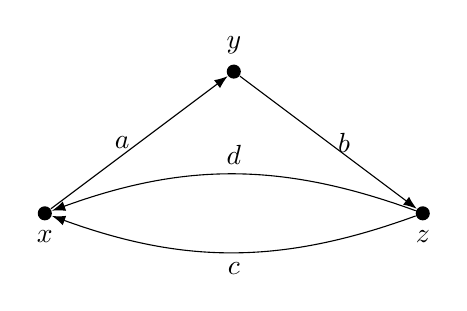
\begin{tikzpicture}[scale=1.2,>=Latex]
			\node[circle,fill=black,inner sep=1.8pt,label=below:\(x\)] (x) at (0,0) {};
			\node[circle,fill=black,inner sep=1.8pt,label=above:\(y\)] (y) at (2,1.5) {};
			\node[circle,fill=black,inner sep=1.8pt,label=below:\(z\)] (z) at (4,0) {};
			
			\draw[->] (x) -- node[left] {\(a\)} (y);
			\draw[->] (y) -- node[right] {\(b\)} (z);
			\draw[->] (z) to[bend left=20] node[below] {\(c\)} (x);
			\draw[->] (z) to[bend right=20] node[above] {\(d\)} (x);
		\end{tikzpicture}
	\end{center}
	
	\subsubsection*{Step 1: The chain groups}
	
	The \(0\)-chains are generated by the vertices:
	\[
	C_0(G)=\mathbb{Z}\langle x,y,z\rangle.
	\]
	
	The \(1\)-chains are generated by the edges:
	\[
	C_1(G)=\mathbb{Z}\langle a,b,c,d\rangle.
	\]
	
	\subsubsection*{Step 2: Compute the boundary map}
	
	By definition,
	\[
	\partial_1(a)=y-x,\qquad
	\partial_1(b)=z-y,\qquad
	\partial_1(c)=x-z,\qquad
	\partial_1(d)=x-z.
	\]
	
	Now let
	\[
	u=\alpha a+\beta b+\gamma c+\delta d \in C_1(G).
	\]
	Then
	\[
	\partial_1(u)
	=
	\alpha(y-x)+\beta(z-y)+\gamma(x-z)+\delta(x-z).
	\]
	Grouping coefficients of \(x,y,z\), we obtain
	\[
	\partial_1(u)
	=
	(-\alpha+\gamma+\delta)x+(\alpha-\beta)y+(\beta-\gamma-\delta)z.
	\]
	
	For \(u\) to be a cycle, we require \(\partial_1(u)=0\), so the coefficients of \(x,y,z\) must vanish:
	\[
	-\alpha+\gamma+\delta=0,
	\qquad
	\alpha-\beta=0,
	\qquad
	\beta-\gamma-\delta=0.
	\]
	
	These equations are equivalent to
	\[
	\alpha=\beta
	\qquad \text{and} \qquad
	\alpha=\gamma+\delta.
	\]
	
	Therefore every cycle has the form
	\[
	u=(\gamma+\delta)a+(\gamma+\delta)b+\gamma c+\delta d.
	\]
	Rearranging,
	\[
	u=\gamma(a+b+c)+\delta(a+b+d).
	\]
	
	Hence
	\[
	\ker(\partial_1)=\mathbb{Z}\langle a+b+c,\;a+b+d\rangle \cong \mathbb{Z}^2.
	\]
	
	Since the graph has no \(2\)-cells,
	\[
	\operatorname{im}(\partial_2)=0.
	\]
	Thus
	\[
	H_1(G)=\ker(\partial_1)\cong \mathbb{Z}^2.
	\]
	
	\subsubsection*{Step 3: Interpreting the generators}
	
	The cycle
	\[
	a+b+c
	\]
	corresponds to the loop
	\[
	x \xrightarrow{a} y \xrightarrow{b} z \xrightarrow{c} x.
	\]
	
	The cycle
	\[
	a+b+d
	\]
	corresponds to the loop
	\[
	x \xrightarrow{a} y \xrightarrow{b} z \xrightarrow{d} x.
	\]
	
	A third cycle is
	\[
	c-d.
	\]
	Indeed,
	\[
	\partial_1(c-d)=\partial_1(c)-\partial_1(d)=(x-z)-(x-z)=0.
	\]
	So \(c-d\) is a cycle. But it is not independent, because
	\[
	(c-d)=(a+b+c)-(a+b+d).
	\]
	Thus it does not contribute a new generator of \(H_1(G)\).
	
	So the graph has exactly two independent loops.
	
	\subsubsection*{Step 4: Compute \(H_0(G)\)}
	
	Because the graph is connected, all vertices become homologous in degree \(0\), so
	\[
	H_0(G)\cong \mathbb{Z}.
	\]
	
	Therefore the full homology of this graph is
	\[
	H_0(G)\cong \mathbb{Z},\qquad
	H_1(G)\cong \mathbb{Z}^2,\qquad
	H_n(G)=0 \text{ for } n\ge 2.
	\]
	
	\subsection{Why signs matter}
	
	The signs in a chain record orientation.
	
	\begin{itemize}[leftmargin=2em]
		\item \(a+b+c\) means we traverse all three edges in their chosen directions.
		\item \(c-d\) means we traverse \(c\) in its chosen direction and \(d\) in the opposite direction.
	\end{itemize}
	
	So homology is not merely counting sets of edges; it is counting algebraically balanced traversals of edges.
	
	\subsection{Cycle condition as a balance law}
	
	A \(1\)-chain is a cycle exactly when its boundary is zero. For graphs, this means that at every vertex,
	\[
	\text{incoming coefficient} = \text{outgoing coefficient}.
	\]
	
	For example:
	\[
	\partial_1(a+b+c)=(y-x)+(z-y)+(x-z)=0,
	\]
	so \(a+b+c\) is a cycle.
	
	But
	\[
	\partial_1(a+b)=(y-x)+(z-y)=z-x\neq 0,
	\]
	so \(a+b\) is not a cycle. It starts at \(x\) and ends at \(z\), so it does not close up.
	
	\subsection{Geometric meaning of \(H_1\)}
	
	The first homology group \(H_1(G)\) measures independent loops in the graph. Since there are no \(2\)-dimensional faces, no loop can be declared trivial by being the boundary of a filled-in region inside the graph.
	
	This is important. In a graph, every independent loop counts.
	
	Thus:
	\[
	\operatorname{rank} H_1(G)=\text{number of independent cycles}.
	\]
	
	\subsection{Geometric meaning of \(H_0\)}
	
	The group \(H_0(G)\) measures connected components. If the graph has \(k\) connected components, then
	\[
	H_0(G)\cong \mathbb{Z}^k.
	\]
	
	In particular:
	\begin{itemize}[leftmargin=2em]
		\item if \(G\) is connected, then \(H_0(G)\cong \mathbb{Z}\);
		\item if \(G\) has two connected components, then \(H_0(G)\cong \mathbb{Z}^2\).
	\end{itemize}
	
	\subsection{More worked examples}
	
	\begin{example}[A single edge]
		Consider the graph
		\[
		x \xrightarrow{a} y.
		\]
		Then
		\[
		C_1=\mathbb{Z}\langle a\rangle,\qquad C_0=\mathbb{Z}\langle x,y\rangle,
		\]
		and
		\[
		\partial_1(a)=y-x.
		\]
		No nonzero multiple of \(a\) has zero boundary, so
		\[
		\ker(\partial_1)=0.
		\]
		Hence
		\[
		H_1(G)=0.
		\]
		The graph is connected, so
		\[
		H_0(G)\cong \mathbb{Z}.
		\]
		So this graph has one connected component and no loops.
	\end{example}
	
	\begin{example}[A triangle]
		Let \(G\) be the cycle
		\[
		x \xrightarrow{a} y \xrightarrow{b} z \xrightarrow{c} x.
		\]
		Then
		\[
		a+b+c
		\]
		is a cycle, and every cycle is an integer multiple of this one. Therefore
		\[
		H_1(G)\cong \mathbb{Z}.
		\]
		Since the graph is connected,
		\[
		H_0(G)\cong \mathbb{Z}.
		\]
		So a triangle has exactly one independent loop.
	\end{example}
	
	\begin{center}
		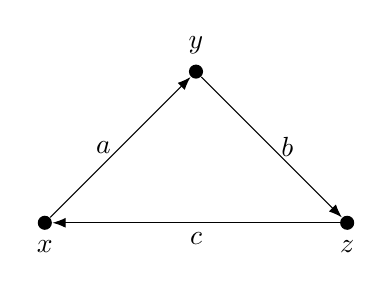
\begin{tikzpicture}[scale=1.2,>=Latex]
			\node[circle,fill=black,inner sep=1.8pt,label=below:\(x\)] (x) at (0,0) {};
			\node[circle,fill=black,inner sep=1.8pt,label=above:\(y\)] (y) at (1.6,1.6) {};
			\node[circle,fill=black,inner sep=1.8pt,label=below:\(z\)] (z) at (3.2,0) {};
			
			\draw[->] (x) -- node[left] {\(a\)} (y);
			\draw[->] (y) -- node[right] {\(b\)} (z);
			\draw[->] (z) -- node[below] {\(c\)} (x);
		\end{tikzpicture}
	\end{center}
	
	\begin{example}[A tree]
		A connected tree has no loops. Therefore
		\[
		H_1(G)=0,
		\qquad
		H_0(G)\cong \mathbb{Z}.
		\]
		This is one of the fundamental characterizations of trees:
		a connected graph is a tree if and only if its first homology group is zero.
	\end{example}
	
	\begin{example}[Two disjoint circles]
		Suppose \(G\) consists of two disconnected loop components. Then the graph has two connected components and two independent loops. Therefore
		\[
		H_0(G)\cong \mathbb{Z}^2,
		\qquad
		H_1(G)\cong \mathbb{Z}^2.
		\]
	\end{example}
	
	\begin{example}[The theta graph]
		The theta graph has two vertices joined by three parallel edges. Topologically it contains two independent loops. Hence
		\[
		H_1(G)\cong \mathbb{Z}^2.
		\]
		Since it is connected,
		\[
		H_0(G)\cong \mathbb{Z}.
		\]
	\end{example}
	
	\subsection{A general formula for finite graphs}
	
	Let \(G\) be a finite graph with
	\begin{itemize}[leftmargin=2em]
		\item \(m\) edges,
		\item \(n\) vertices,
		\item \(k\) connected components.
	\end{itemize}
	
	Then
	\[
	\operatorname{rank} H_1(G)=m-n+k.
	\]
	Equivalently,
	\[
	H_1(G)\cong \mathbb{Z}^{\,m-n+k}.
	\]
	
	This number
	\[
	\beta_1(G)=m-n+k
	\]
	is called the \emph{first Betti number} of the graph.
	
	\begin{remark}
		If the graph is connected, so \(k=1\), then
		\[
		\operatorname{rank} H_1(G)=m-n+1.
		\]
		For a tree, we have \(m=n-1\), so \(H_1(G)=0\). Every time we add one extra edge to a connected graph, we create one new independent cycle, and the rank of \(H_1\) increases by \(1\).
	\end{remark}
	
	\subsection{Applying the formula to the main example}
	
	In our graph with vertices \(\{x,y,z\}\) and edges \(\{a,b,c,d\}\), we have
	\[
	m=4,\qquad n=3,\qquad k=1.
	\]
	Therefore
	\[
	\operatorname{rank} H_1(G)=m-n+k=4-3+1=2.
	\]
	Hence
	\[
	H_1(G)\cong \mathbb{Z}^2,
	\]
	exactly as found by direct computation.
	
	\subsection{Linear algebra viewpoint}
	
	If we list the vertices and edges, then the map
	\[
	\partial_1:C_1(G)\to C_0(G)
	\]
	is represented by the incidence matrix of the graph. Thus graph homology can be computed by ordinary linear algebra over \(\mathbb{Z}\):
	
	\begin{itemize}[leftmargin=2em]
		\item the cycles are the elements of \(\ker(\partial_1)\),
		\item for graphs, \(H_1(G)=\ker(\partial_1)\),
		\item \(H_0(G)\) describes connected components.
	\end{itemize}
	
	So graph homology is a very concrete bridge between topology and algebra.
	
	\subsection{Important conceptual point about ``holes''}
	
	When one says that a graph has ``holes,'' this does \emph{not} simply mean bounded regions in some particular drawing of the graph in the plane. A graph can be drawn in many different ways, but its homology does not change.
	
	Homology counts independent loops in the graph as a topological space. In a graph, a ``hole'' means an independent cycle that is not the boundary of a \(2\)-dimensional piece. Since graphs have no \(2\)-dimensional pieces, every independent cycle contributes to \(H_1\).
	
	\subsection{Final summary}
	
	For a finite graph \(G\):
	\begin{align*}
		H_0(G) &\cong \mathbb{Z}^{\,\#\text{connected components}},\\[4pt]
		H_1(G) &\cong \mathbb{Z}^{\,m-n+k},\\[4pt]
		H_r(G) &=0 \qquad \text{for all } r\ge 2.
	\end{align*}
	
	In the main example with vertices \(x,y,z\) and edges \(a,b,c,d\),
	\[
	H_0(G)\cong \mathbb{Z},
	\qquad
	H_1(G)\cong \mathbb{Z}^2,
	\qquad
	H_n(G)=0 \text{ for } n\ge 2.
	\]
	
	So the graph is connected and has exactly two independent loops.


\section{Simplices, orientations, chains, boundaries, and cycles}

This section develops the basic language of simplicial homology. The goal is to explain clearly what simplices are, how orientations are assigned, how chains are formed, how the boundary operator works, and how cycles and boundaries lead to homology groups.

\subsection{Simplices: geometric building blocks}

A \emph{\(k\)-simplex} is the simplest possible \(k\)-dimensional geometric object.

\begin{itemize}
	\item A \(0\)-simplex is a point.
	\item A \(1\)-simplex is a line segment.
	\item A \(2\)-simplex is a filled triangle.
	\item A \(3\)-simplex is a filled tetrahedron.
\end{itemize}

More formally, if \(v_0,\dots,v_k\) are affinely independent points in some Euclidean space, then the \(k\)-simplex spanned by them is
\[
[v_0,\dots,v_k]
=
\left\{
\sum_{i=0}^{k}\lambda_i v_i
\;\middle|\;
\lambda_i\ge 0,\ \sum_{i=0}^{k}\lambda_i=1
\right\}.
\]
This is the convex hull of the vertices \(v_0,\dots,v_k\).

\subsubsection*{Examples}

\begin{itemize}
	\item The simplex \([v_0]\) is just the point \(v_0\).
	\item The simplex \([v_0,v_1]\) is the segment joining \(v_0\) and \(v_1\).
	\item The simplex \([v_0,v_1,v_2]\) is the filled-in triangle with those three vertices.
	\item The simplex \([v_0,v_1,v_2,v_3]\) is the filled tetrahedron.
\end{itemize}

It is important that simplices are \emph{filled in}. Thus a \(2\)-simplex is not merely the boundary triangle; it includes the whole triangular region.

\subsection{Faces of a simplex}

A \emph{face} of a simplex is obtained by choosing some of its vertices and taking their convex hull.

For example, if \(\sigma=[v_0,v_1,v_2]\) is a \(2\)-simplex, then its faces are:
\begin{itemize}
	\item the three vertices \([v_0]\), \([v_1]\), \([v_2]\),
	\item the three edges \([v_0,v_1]\), \([v_0,v_2]\), \([v_1,v_2]\),
	\item the simplex itself \([v_0,v_1,v_2]\).
\end{itemize}

If \(\tau\) is a face of \(\sigma\), we write \(\tau\le \sigma\).

\subsection{Simplicial complexes}

A \emph{simplicial complex} \(K\) is a collection of simplices such that:

\begin{enumerate}
	\item every face of a simplex in \(K\) also belongs to \(K\),
	\item the intersection of any two simplices in \(K\) is either empty or a common face of both.
\end{enumerate}

So a simplicial complex is built by gluing simplices together along shared faces in a consistent way.

\subsubsection*{Examples of simplicial complexes}

\begin{itemize}
	\item A graph is a simplicial complex consisting only of vertices and edges.
	\item A triangulated polygon is a simplicial complex made of vertices, edges, and triangles.
	\item The boundary of a tetrahedron is a simplicial complex made of four triangles glued along edges; topologically it is a sphere \(S^2\).
\end{itemize}

\subsection{Orientations of simplices}

A key idea in simplicial homology is that simplices are given \emph{orientations}.

\begin{definition}[Orientation of a simplex]
	An orientation of a \(k\)-simplex with vertices \(v_0,\dots,v_k\) is given by an ordering
	\[
	(v_0,\dots,v_k),
	\]
	where two orderings define the same orientation if and only if they differ by an even permutation.
\end{definition}

Thus each simplex has exactly two orientations.

Changing two vertices reverses the orientation. More generally, an odd permutation changes the orientation sign.

\subsubsection*{Examples of orientation}

\paragraph{A \(1\)-simplex.}
For an edge with vertices \(v_0,v_1\), the two possible orientations are
\[
(v_0,v_1)
\qquad \text{and} \qquad
(v_1,v_0).
\]
These are opposites. Geometrically, choosing an orientation of an edge means choosing a direction along the edge.

\paragraph{A \(2\)-simplex.}
For a triangle with vertices \(v_0,v_1,v_2\), the orderings
\[
(v_0,v_1,v_2),\quad (v_1,v_2,v_0),\quad (v_2,v_0,v_1)
\]
define one orientation, while
\[
(v_0,v_2,v_1),\quad (v_2,v_1,v_0),\quad (v_1,v_0,v_2)
\]
define the opposite orientation.

Geometrically, this corresponds to choosing which direction around the triangle counts as positive, for example counterclockwise versus clockwise.

\subsection{Orientation signs in chain groups}

In simplicial homology, opposite orientations differ by a minus sign. Thus we impose the relation
\[
(v_0,\dots,v_k)=\operatorname{sgn}(\pi)\,(v_{\pi(0)},\dots,v_{\pi(k)})
\]
for every permutation \(\pi\in S_{k+1}\).

In particular,
\[
(v_0,v_1)=-(v_1,v_0),
\]
and
\[
(v_0,v_1,v_2)=-(v_1,v_0,v_2).
\]

So an oriented simplex and the same simplex with reverse orientation are negatives of one another.

\subsection{Chains}

Let \(K\) be a simplicial complex.

\begin{definition}[Simplicial \(k\)-chain]
	A \emph{simplicial \(k\)-chain} is a finite formal sum
	\[
	c=\sum_{i=1}^{N} n_i \sigma_i,
	\]
	where each \(n_i\in \mathbb{Z}\) and each \(\sigma_i\) is an oriented \(k\)-simplex.
\end{definition}

The set of all \(k\)-chains forms an abelian group, denoted \(C_k(K)\). This is the free abelian group generated by the oriented \(k\)-simplices, modulo the relation that reversing orientation changes the sign.

\subsubsection*{Examples of chains}

\paragraph{Example 1: \(0\)-chains.}
If the vertices are \(v_0,v_1,v_2\), then a typical \(0\)-chain is
\[
2v_0-3v_1+5v_2.
\]

\paragraph{Example 2: \(1\)-chains.}
If the oriented edges are \((v_0,v_1)\), \((v_1,v_2)\), and \((v_0,v_2)\), then
\[
(v_0,v_1)+(v_1,v_2)-(v_0,v_2)
\]
is a \(1\)-chain.

\paragraph{Example 3: \(2\)-chains.}
If \(K\) contains triangles \((v_0,v_1,v_2)\) and \((v_0,v_2,v_3)\), then
\[
(v_0,v_1,v_2) - 2(v_0,v_2,v_3)
\]
is a \(2\)-chain.

A chain need not represent a closed geometric object. It is simply an algebraic combination of simplices.

\subsection{Choosing a basis for \(C_k(K)\)}

To make \(C_k(K)\) concrete, one usually chooses one orientation for each \(k\)-simplex. Then those oriented simplices form a basis for the free abelian group \(C_k(K)\).

A standard method is to choose an ordering of all vertices of the complex and then orient each simplex by the induced order of its vertices.

For instance, if the global vertex order is
\[
v_0 < v_1 < v_2 < v_3,
\]
then the simplex \([v_0,v_2,v_3]\) is represented by the oriented simplex
\[
(v_0,v_2,v_3).
\]

\subsection{The boundary operator}

The boundary operator extracts the oriented faces of a simplex.

\begin{definition}[Boundary map]
	Let \(\sigma=(v_0,\dots,v_k)\) be an oriented \(k\)-simplex. Its boundary is defined by
	\[
	\partial_k(\sigma)
	=
	\sum_{i=0}^{k} (-1)^i (v_0,\dots,\widehat{v_i},\dots,v_k),
	\]
	where the hat means that the vertex \(v_i\) is omitted.
\end{definition}

This formula extends linearly to all \(k\)-chains:
\[
\partial_k\left(\sum_i n_i \sigma_i\right)=\sum_i n_i\,\partial_k(\sigma_i).
\]

Thus
\[
\partial_k : C_k(K)\to C_{k-1}(K)
\]
is a group homomorphism.

\subsubsection*{Low-dimensional boundary formulas}

\paragraph{Boundary of a vertex.}
A \(0\)-simplex has no lower-dimensional faces, so
\[
\partial_0(v)=0.
\]

\paragraph{Boundary of an oriented edge.}
For a \(1\)-simplex \((v_0,v_1)\),
\[
\partial_1(v_0,v_1)=(v_1)-(v_0)=v_1-v_0.
\]
So the boundary of an oriented edge is its endpoint minus its starting point.

\paragraph{Boundary of an oriented triangle.}
For a \(2\)-simplex \((v_0,v_1,v_2)\),
\[
\partial_2(v_0,v_1,v_2)
=
(v_1,v_2)-(v_0,v_2)+(v_0,v_1).
\]
Equivalently,
\[
\partial_2(v_0,v_1,v_2)
=
(v_0,v_1)+(v_1,v_2)+(v_2,v_0),
\]
since
\[
-(v_0,v_2)=(v_2,v_0).
\]
So the boundary of an oriented triangle is the sum of its oriented edges, traversed consistently around the boundary.

\paragraph{Boundary of an oriented tetrahedron.}
For a \(3\)-simplex \((v_0,v_1,v_2,v_3)\),
\[
\partial_3(v_0,v_1,v_2,v_3)
=
(v_1,v_2,v_3)
-(v_0,v_2,v_3)
+(v_0,v_1,v_3)
-(v_0,v_1,v_2).
\]
Thus the boundary of a tetrahedron is the alternating sum of its four triangular faces.

\subsection{Concrete examples of boundaries}

\subsubsection*{Example 1: boundary of an edge}

Let \(e=(v_0,v_1)\). Then
\[
\partial_1(e)=v_1-v_0.
\]
If we reverse the orientation, then
\[
\partial_1(v_1,v_0)=v_0-v_1=-(v_1-v_0).
\]
So reversing orientation reverses the sign of the boundary.

\subsubsection*{Example 2: boundary of a triangle}

Let \(\sigma=(v_0,v_1,v_2)\). Then
\[
\partial_2(\sigma)
=
(v_1,v_2)-(v_0,v_2)+(v_0,v_1).
\]
This can be pictured as the three sides of the triangle, taken with compatible orientation around the boundary.

If instead we take the opposite orientation \((v_0,v_2,v_1)\), then
\[
\partial_2(v_0,v_2,v_1)=-\partial_2(v_0,v_1,v_2).
\]

\subsubsection*{Example 3: sum of two triangles sharing an edge}

Suppose a complex contains two oriented triangles
\[
\sigma_1=(v_0,v_1,v_2),
\qquad
\sigma_2=(v_0,v_2,v_3).
\]
Then
\[
\partial_2(\sigma_1)
=
(v_1,v_2)-(v_0,v_2)+(v_0,v_1),
\]
and
\[
\partial_2(\sigma_2)
=
(v_2,v_3)-(v_0,v_3)+(v_0,v_2).
\]
Adding them gives
\[
\partial_2(\sigma_1+\sigma_2)
=
(v_0,v_1)+(v_1,v_2)+(v_2,v_3)-(v_0,v_3).
\]
The edge \((v_0,v_2)\) cancels with \(-(v_0,v_2)\). Geometrically, the common interior edge disappears from the boundary, leaving only the outer boundary of the union.

This is one of the most important geometric features of the boundary operator: interior faces cancel.

\subsection{Cycles and boundaries}

\begin{definition}[Cycles]
	The subgroup
	\[
	Z_k(K):=\ker(\partial_k)\subseteq C_k(K)
	\]
	is called the group of \emph{\(k\)-cycles}.
\end{definition}

So a \(k\)-cycle is a \(k\)-chain whose boundary is zero.

\begin{definition}[Boundaries]
	The subgroup
	\[
	B_k(K):=\operatorname{im}(\partial_{k+1})\subseteq C_k(K)
	\]
	is called the group of \emph{\(k\)-boundaries}.
\end{definition}

So a \(k\)-boundary is a \(k\)-chain that is itself the boundary of some \((k+1)\)-chain.

\subsubsection*{Intuition}

\begin{itemize}
	\item A cycle is something closed: it has no boundary.
	\item A boundary is something that comes from the boundary of a higher-dimensional object.
\end{itemize}

Not every cycle is necessarily a boundary. The difference between cycles and boundaries is precisely what homology measures.

\subsection{Examples of cycles and boundaries}

\subsubsection*{Example 1: a loop in a graph}

Let a simplicial complex consist of three vertices \(v_0,v_1,v_2\) and three edges forming a triangle, but with no filled interior. Consider the \(1\)-chain
\[
c=(v_0,v_1)+(v_1,v_2)+(v_2,v_0).
\]
Then
\[
\partial_1(c)
=
(v_1-v_0)+(v_2-v_1)+(v_0-v_2)=0.
\]
So \(c\) is a \(1\)-cycle.

Since the complex has no \(2\)-simplices, \(c\) cannot be the boundary of any \(2\)-chain. Thus \(c\) is a cycle but not a boundary.

This is the algebraic expression of a genuine \(1\)-dimensional hole.

\subsubsection*{Example 2: the boundary of a filled triangle}

Now suppose the same triangle is filled in, so the complex contains the \(2\)-simplex \((v_0,v_1,v_2)\). Then
\[
\partial_2(v_0,v_1,v_2)
=
(v_0,v_1)+(v_1,v_2)+(v_2,v_0).
\]
Thus the same loop is now a boundary.

So in the filled triangle, the outer loop does not represent a hole; it bounds the \(2\)-simplex.

\subsubsection*{Example 3: boundary of a tetrahedron}

Let \(K\) be the boundary complex of a tetrahedron. The sum of its four triangular faces is a \(2\)-cycle: the boundary of the whole closed surface is zero. But it is not a boundary inside this complex, because the \(3\)-simplex filling the tetrahedron is not included.

If instead the full tetrahedron is included as a \(3\)-simplex, then the sum of the four faces becomes a boundary:
\[
\partial_3(v_0,v_1,v_2,v_3)
=
(v_1,v_2,v_3)
-(v_0,v_2,v_3)
+(v_0,v_1,v_3)
-(v_0,v_1,v_2).
\]

\subsection{Why \(\partial^2=0\)}

A fundamental fact is that
\[
\partial_{k-1}\circ \partial_k = 0
\qquad \text{for every } k\ge 1.
\]
In words:
\[
\text{the boundary of a boundary is always zero.}
\]

This is the reason boundaries are always cycles:
\[
B_k(K)\subseteq Z_k(K).
\]

\subsubsection*{Example: boundary of the boundary of a triangle}

Let \(\sigma=(v_0,v_1,v_2)\). Then
\[
\partial_2(\sigma)
=
(v_1,v_2)-(v_0,v_2)+(v_0,v_1).
\]
Apply \(\partial_1\):
\begin{align*}
	\partial_1\partial_2(\sigma)
	&=
	\partial_1(v_1,v_2)-\partial_1(v_0,v_2)+\partial_1(v_0,v_1)\\
	&=
	(v_2-v_1)-(v_2-v_0)+(v_1-v_0)\\
	&=0.
\end{align*}

Each vertex appears twice with opposite signs, so everything cancels.

\subsubsection*{Geometric meaning}

If you take the boundary of a triangle, you get its three edges.  
If you then take the boundary of those edges, you get the three vertices, but every vertex appears once with a plus sign and once with a minus sign. So they cancel.

Likewise, the boundary of a tetrahedron is four triangles, and the boundary of those four triangles is zero because every edge appears twice with opposite orientations.

\subsection{Homology groups}

Because \(B_k(K)\subseteq Z_k(K)\), we can form the quotient
\[
H_k(K):=Z_k(K)/B_k(K).
\]
This is the \emph{\(k\)-th simplicial homology group}.

It measures \(k\)-cycles modulo those \(k\)-cycles that are boundaries.

\subsubsection*{Interpretation}

\begin{itemize}
	\item \(H_0(K)\) measures connected components.
	\item \(H_1(K)\) measures loops that do not bound triangles or higher \(2\)-chains.
	\item \(H_2(K)\) measures closed surfaces that do not bound \(3\)-chains.
\end{itemize}

So homology detects genuine holes.

\subsection{Two basic examples of homology}

\subsubsection*{Example 1: a hollow triangle}

Let \(K\) consist of the three edges and three vertices of a triangle, but no \(2\)-simplex.

Then the \(1\)-chain
\[
c=(v_0,v_1)+(v_1,v_2)+(v_2,v_0)
\]
is a cycle. Since there is no \(2\)-simplex, it is not a boundary. Therefore it defines a nonzero class in \(H_1(K)\).

So
\[
H_1(K)\cong \mathbb{Z}.
\]

\subsubsection*{Example 2: a filled triangle}

Now let \(K\) contain the \(2\)-simplex \((v_0,v_1,v_2)\) as well. Then
\[
c=\partial_2(v_0,v_1,v_2),
\]
so \(c\in B_1(K)\). Thus it becomes trivial in homology:
\[
[c]=0 \in H_1(K).
\]

So the filled triangle has no \(1\)-dimensional hole:
\[
H_1(K)=0.
\]

\subsection{A useful viewpoint: algebra mirrors geometry}

The algebraic definitions may look formal at first, but they mirror geometry exactly:

\begin{itemize}
	\item simplices are the geometric pieces,
	\item orientations keep track of direction and sign,
	\item chains are formal sums of these pieces,
	\item the boundary operator extracts the oriented boundary,
	\item cycles are closed objects,
	\item boundaries are those closed objects that come from higher-dimensional pieces,
	\item homology records which cycles are not boundaries.
\end{itemize}

\subsection{Final summary}

For a simplicial complex \(K\):

\begin{itemize}
	\item \(C_k(K)\) is the free abelian group on oriented \(k\)-simplices,
	\item the boundary operator is
	\[
	\partial_k(v_0,\dots,v_k)
	=
	\sum_{i=0}^{k}(-1)^i(v_0,\dots,\widehat{v_i},\dots,v_k),
	\]
	\item the \(k\)-cycles are
	\[
	Z_k(K)=\ker(\partial_k),
	\]
	\item the \(k\)-boundaries are
	\[
	B_k(K)=\operatorname{im}(\partial_{k+1}),
	\]
	\item the \(k\)-th homology group is
	\[
	H_k(K)=Z_k(K)/B_k(K).
	\]
\end{itemize}

The fundamental principle is:

\[
\partial^2=0,
\qquad\text{so every boundary is a cycle.}
\]

Homology measures exactly the cycles that are not boundaries, hence the genuine holes of the space.

\end{document}
